\documentclass[11pt,a4paper]{article}
\usepackage[margin=24mm]{geometry}
\usepackage{amsmath,amssymb}
\usepackage{booktabs}
\usepackage[T1]{fontenc}
\usepackage{lmodern}
\usepackage{microtype}
\usepackage{xcolor}
\usepackage{listings}
\usepackage{tikz}
\usepackage[hidelinks]{hyperref}
\usetikzlibrary{positioning,arrows.meta,fit,backgrounds,calc}

\definecolor{ink}{HTML}{1A1A1A}
\definecolor{grey}{HTML}{5F5B54}
\definecolor{pale}{HTML}{F5F3EE}
\definecolor{tensor}{HTML}{1F6F4A}
\definecolor{seq}{HTML}{1F4E8C}
\definecolor{prod}{HTML}{9C3B1B}
\definecolor{sum}{HTML}{6B4E9C}
\definecolor{warn}{HTML}{9C3B1B}

\lstdefinestyle{ts}{basicstyle=\ttfamily\footnotesize, showstringspaces=false,
  columns=fullflexible, keepspaces=true, breaklines=true,
  commentstyle=\color{grey}\itshape, keywordstyle=\color{ink}\bfseries,
  backgroundcolor=\color{pale}, frame=none, xleftmargin=4mm, framexleftmargin=4mm}
\lstset{style=ts}

\tikzset{
  srv/.style={draw=ink, fill=white, rounded corners=2pt, inner sep=3.4pt,
              font=\scriptsize\ttfamily, minimum height=5.6mm},
  plan/.style={srv, fill=pale, font=\scriptsize\ttfamily\bfseries},
  op/.style={circle, draw, inner sep=0.6pt, minimum size=6.4mm, font=\footnotesize\bfseries},
  ar/.style={-{Stealth[length=1.8mm]}, semithick, color=grey},
  lbl/.style={font=\tiny\itshape, color=grey},
  capt/.style={font=\scriptsize\bfseries},
  subt/.style={font=\tiny\itshape, color=grey},
}

\title{\vspace{-2em}\textbf{\texttt{stalin}}\\[2mm]
  \large The First Five-Year Plan as a container}
\author{\normalsize Documentation}
\date{\normalsize\today}

\begin{document}
\maketitle
\thispagestyle{empty}

\begin{abstract}
\noindent
\texttt{stalin} is a resource-allocation game about Soviet industrialisation,
built on the container algebra of Neil Ghani's \emph{Containers for Typed
Agentic AI}. It runs as five HTTP servers exchanging JSON. This document
describes the game and how to win it; revises the parts of the framework it
uses; draws the game as a composite of the four combinators; and then sets out
what the implementation actually guarantees --- which turns out to be less than
it looks, in a way that is the game's own subject.
\end{abstract}

\tableofcontents
\newpage

\section{The game}

You are not Stalin. You are the Plan --- Gosplan, in a building in Moscow,
deciding each year what a hundred and twenty million people will do with
themselves. You issue five plans, and then you are judged twice.

\subsection{The country you are given}

It grows grain and almost nothing else. In 1928 there are 120 people: 105 on
the land, 8 in a small steel mill, 7 on a railway that reaches some of the
places it should. There are no tractors, no foreign engineers, 10 tonnes of
steel and no hard currency. Everyone eats, whether or not they grow anything.

\subsection{What you are trying to do}

Two things at once, and they pull against each other.

\textbf{Mechanise.} A peasant with a tractor out-produces a peasant with a
back, so tractors let you take hands off the land and put them in the mills
without the country going hungry. To build tractors you need a works; to build
the works you need steel and a German engineer; the engineer wants hard
currency; hard currency comes from selling grain abroad --- grain the villages
were going to eat. That circle is the game.

\textbf{Survive 1941.} You do not fight that war, but you pay for it here.
Steel put by for armaments never becomes a tractor and never earns a rouble. It
buys exactly one thing: soldiers who come home. You never conscript during the
plan; in 1941 the country calls up precisely as many men as the armaments
require, and no more --- so the size of the army, and therefore the dead, is
decided years earlier by how much steel you set aside.

\subsection{A year is two turns}

\begin{center}
\begin{tabular}{@{}ll@{}}
\toprule
\textbf{spring} & where the hands go, and how hard the villages are squeezed \\
\textbf{autumn} & the harvest is in and graded; you dispose of it \\
\bottomrule
\end{tabular}
\end{center}

\noindent The split is the point. In spring you fix the labour allocation and
the procurement quota \emph{before you know the weather}. A quota set in March
against a harvest that fails in August is not a game mechanic; it is how a
famine is administered. By autumn the grade is known --- \texttt{failure},
\texttt{poor}, \texttt{adequate}, \texttt{bumper} --- and it decides which
export decisions are even available to you. Five years, ten turns.

\subsection{The score}

One number: how many of your people die. Starved and fallen, added together.
Win the war, and lose as few as you can.

The game reports both halves separately and refuses to combine them for you
beyond the sum. It also reports whether you mechanised --- whether the final
harvest beat 1928's with fewer hands --- and does not fold that into the score
at all.

\section{Strategies}

Seven representative plans, same seed. Letters are what a player types; a
sequence of ten letters is a whole game.

\begin{center}
\footnotesize
\begin{tabular}{@{}llrrrrl@{}}
\toprule
strategy & letters & tractors & armaments & starved & fallen & outcome \\
\midrule
gentle arms      & \texttt{AJBEBJAJAJ} &  2 & 89 &  5 &  4 & won, \textbf{9} dead \\
brutalist mech.  & \texttt{CMKEBIBJNJ} & 22 & 98 & 15 &  3 & won, \textbf{18} dead \\
no railway       & \texttt{KABEBIBJAJ} & 22 & 82 & 25 &  4 & won, \textbf{29} dead \\
partial arms     & \texttt{CABEBINJAA} & 42 & 34 & 21 & 14 & won, \textbf{35} dead \\
totally brutal   & \texttt{KJBEAJBJAJ} &  2 & 78 & 44 &  5 & won, \textbf{49} dead \\
bought tractors  & \texttt{AMAMAFAMAF} & 18 &  0 &  3 & 57 & \textbf{lost} \\
never armed      & \texttt{CAKEBINIAI} & 62 &  0 & 15 & 52 & \textbf{lost} \\
\bottomrule
\end{tabular}
\end{center}

\subsection{Reading the table}

\textbf{Never arming loses.} A beautiful mechanised country --- 62 tractors,
the largest harvest on the board --- falls in 1941, because 120 men with
nothing to fire cannot reach the enemy's strength.

\textbf{Buying tractors abroad is the humane road, and it is fatal.} Three
people starve, the fewest of any line. But imported tractors build no mill, no
engineers, and no steel, so there is nothing to arm with. The cheap road is the
trap.

\textbf{Partial armaments wins and bleeds.} 34 tonnes put by is enough to win
and not enough to win cheaply: 14 fallen against the best line's 3. The war
curve is smooth, so half an army is a victory paid for in men.

\textbf{The railway comes before the steel.} Grain the railway cannot move rots
at the sidings. A total quota with no track to carry it starves 25 people for
nothing --- worse than the same brutality with a railway.

\textbf{The two orderings disagree.} Ranked by \emph{soldiers} lost, brutalist
mechanisation is the best plan on the board: 3 fallen, because it ends holding
98 tonnes of armaments, more than any other line, and an army small enough to
carry them. Ranked by \emph{everyone} lost it comes second, because the fifteen
it starved outnumber the one soldier it saved. The game holds both numbers and
declines to say which is the real one.

\subsection{The plan the game is built around, and the one that beats it}

The design intent is that \emph{brutalist mechanisation} should be optimal:
starve the villages early, spend it on rail, engineers and tractors, then turn
the surplus into an army. It is morally uncomfortable and it should win.

It does not. \texttt{AJBEBJAJAJ} --- found by machine search over the menu, not
by hand --- wins for 9 dead by doing almost nothing: put hands in the mill, buy
the Germans once, then smelt straight into armaments for three years. No
railway, no tractors on purpose, no famine beyond the baseline five who die
whatever you do.

The reason is a dependency length rather than a number:

\begin{center}
\footnotesize
\begin{tabular}{@{}llr@{}}
\toprule
& mill workforce, 1928--32 & armaments \\
\midrule
brutalist mechanisation & 8, 8, 16, 23, \textbf{45} & 98, first built in 1932 \\
gentle arms             & 8, 15, 22, 21, 20        & 89, first built in 1929 \\
\bottomrule
\end{tabular}
\end{center}

\noindent The mechanised economy matures in 1932, and then the plan ends. Its
chain is rail $\to$ export $\to$ engineers $\to$ works $\to$ tractors $\to$
freed hands $\to$ mill $\to$ steel $\to$ armaments: nine links, each costing at
least one turn, against ten turns in the plan. The gentle line skips six of
them and spends four years arming instead of one.

This is recorded as a failing test in \texttt{calibrate.ts} rather than
quietly redefined. Seven of the eight design criteria hold across every seed
tried; this is the eighth.

\section{Ghani's containers, revised}

Three ideas, in the order the note develops them.

\subsection{\S3 --- a container is a dependent type}

A container is a pair $(P, R)$:

\begin{center}
$P : \mathrm{Type}$ \qquad the \emph{prompts}, or shapes\\[1mm]
$R : P \to \mathrm{Type}$ \qquad the \emph{positions}: for each prompt, the type of valid replies
\end{center}

\noindent and an inhabitant of the interface is a dependent function
$(p : P) \to R\,p$. The content of that dependency is Ghani's observation that
event-driven programming ``has a feature that turns out to be exactly a
dependent type'': \emph{which responses are appropriate depends on which event
arrived}. Note what is absent --- no loops, no callbacks, no concurrency. Strip
the event loop away and the container is what remains.

A game is a container. $P$ is the situations you can be in; $R\,s$ is the moves
legal at $s$. A player is $(s : P) \to R\,s$. That is not an analogy: it is the
same type.

\subsection{\S4 --- morphisms, or how one container calls another}

A morphism $(P,R) \to (Q,T)$ is a pair:

\begin{center}
$u : P \to Q$ \qquad \emph{delegate}: turn my prompt into one for the level below\\[1mm]
$f : (p : P) \to T\,(u\,p) \to R\,p$ \qquad \emph{amalgamate}: turn their reply into mine
\end{center}

\noindent Control flows \emph{down} through $u$; data flows \emph{up} through
$f$. This is worth dwelling on, because it is exactly the shape of a command
economy --- and, in a game about one, that is not a coincidence but the reason
the fit is good. Gosplan does not do the harvesting. It converts ``feed the
towns'' into ``Narkomzem: reap'', and converts the reply back into a number for
its own ledger.

\subsection{\S5 --- the four combinators}

\begin{center}
\footnotesize
\begin{tabular}{@{}cll@{}}
\toprule
& \textbf{shapes} & \textbf{positions} \\
\midrule
$+$ \ sum        & disjoint union: one side or the other & each keeps its own \\
$\boxtimes$ \ tensor  & multiply: a prompt for each side  & multiply: a reply from each \\
$\lhd$ \ sequential   & a dependent pair $(s \mathbin{**} R\,s \to S')$ & a pair of replies \\
$\times$ \ product    & multiply: prompt both              & \emph{sum}: exactly one answers \\
\bottomrule
\end{tabular}
\end{center}

\noindent The distinction that does the most work here is $\boxtimes$ against
$\times$. Both ask everybody. The tensor requires \emph{all} of them to answer;
the product requires exactly \emph{one}. Same shapes, different positions.

$\lhd$ is the subtle one. Its shape is not a pair of prompts but a first prompt
\emph{together with a function} choosing the second from the first's reply. So
the second question is not knowable when the first is asked --- which is what
makes it sequential rather than parallel, and what makes it hard to type.

\section{The game, as a composite}

\begin{center}
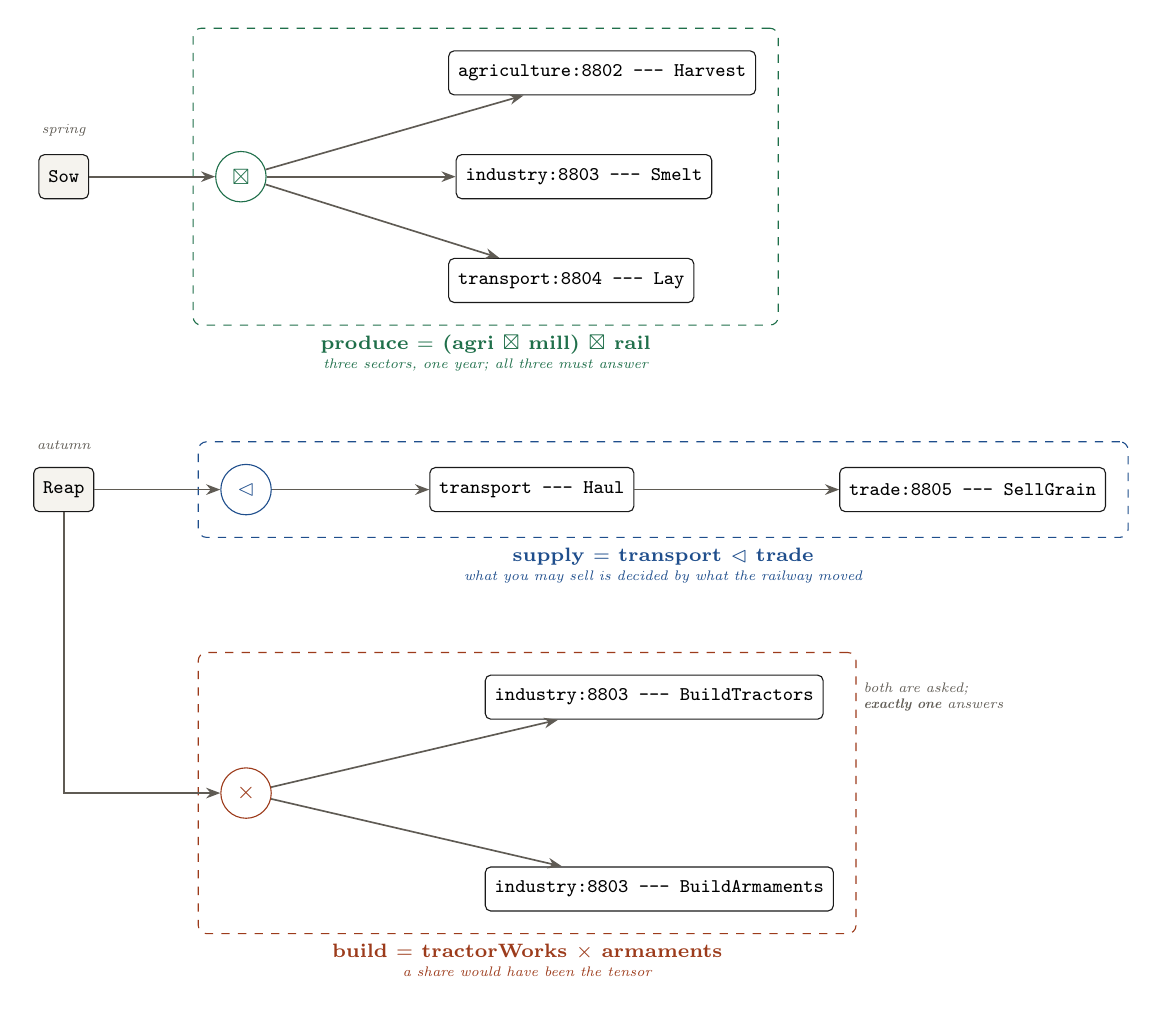
\begin{tikzpicture}

% --- SPRING: tensor ---
\node[plan] (sow) {Sow};
\node[lbl, above=1mm of sow] {spring};
\node[op, draw=tensor, text=tensor] (t1) [right=16mm of sow] {$\boxtimes$};
\node[srv] (agri)  [above right=8mm and 24mm of t1] {agriculture:8802 --- Harvest};
\node[srv] (mill)  [right=24mm of t1]               {industry:8803 --- Smelt};
\node[srv] (rail)  [below right=8mm and 24mm of t1] {transport:8804 --- Lay};
\draw[ar] (sow) -- (t1);
\draw[ar] (t1) -- node[lbl, pos=0.45, above, sloped]{} (agri);
\draw[ar] (t1) -- (mill);
\draw[ar] (t1) -- node[lbl, pos=0.45, below, sloped]{} (rail);
\begin{scope}[on background layer]
\node[fit=(t1)(agri)(mill)(rail), draw=tensor, dashed, rounded corners=3pt,
      inner sep=2.8mm, label={[capt, text=tensor, align=center]below:%
      produce $=$ (agri $\boxtimes$ mill) $\boxtimes$ rail\\[-0.4mm]
      {\normalfont\itshape\tiny three sectors, one year; all three must answer}}] {};
\end{scope}

% --- AUTUMN: seq ---
\node[plan] (reap) [below=34mm of sow] {Reap};
\node[lbl, above=1mm of reap] {autumn};
\node[op, draw=seq, text=seq] (s1) [right=16mm of reap] {$\lhd$};
\node[srv] (rail2) [right=20mm of s1]    {transport --- Haul};
\node[srv] (trade) [right=26mm of rail2] {trade:8805 --- SellGrain};
\draw[ar] (reap) -- (s1);
\draw[ar] (s1) -- (rail2);
\draw[ar] (rail2) -- (trade);
\begin{scope}[on background layer]
\node[fit=(s1)(rail2)(trade), draw=seq, dashed, rounded corners=3pt,
      inner sep=2.8mm, label={[capt, text=seq, align=center]below:%
      supply $=$ transport $\lhd$ trade\\[-0.4mm]
      {\normalfont\itshape\tiny what you may sell is decided by what the railway moved}}] {};
\end{scope}

% --- PRODUCT ---
\node[op, draw=prod, text=prod] (p1) [below=32mm of s1] {$\times$};
\node[srv] (tract) [above right=7mm and 28mm of p1] {industry:8803 --- BuildTractors};
\node[srv] (arms)  [below right=7mm and 28mm of p1] {industry:8803 --- BuildArmaments};
\draw[ar] (reap) |- (p1);
\draw[ar] (p1) -- (tract);
\draw[ar] (p1) -- (arms);
\node[subt, right=4mm of tract, align=left, text width=26mm]
  {both are asked;\\\textbf{exactly one} answers};
\begin{scope}[on background layer]
\node[fit=(p1)(tract)(arms), draw=prod, dashed, rounded corners=3pt,
      inner sep=2.8mm, label={[capt, text=prod, align=center]below:%
      build $=$ tractorWorks $\times$ armaments\\[-0.4mm]
      {\normalfont\itshape\tiny a share would have been the tensor}}] {};
\end{scope}

\end{tikzpicture}
\end{center}

\subsection{Where the sum is, and is not}

$+$ is never built as a composite. There is no \texttt{sumC(\dots)} call in the
game, and it would be an overstatement to claim one. Routing appears instead as
each container's own \emph{shape type} --- a tagged union
$\{\texttt{Harvest}\} + \{\texttt{Winter}\} + \dots$ is a coproduct --- and its
eliminator is the \texttt{switch} in every server's dispatch. Real work, in the
place \S3 always put it; but not a use of the combinator.

\subsection{Two that were removed}

While the railway to the port was narrow, the sale was a \emph{product} (grain
\emph{or} steel, one contract) and became a \emph{tensor} once enough track was
laid (ship both) --- rail capacity choosing between $\times$ and $\boxtimes$,
\S5's own distinction used as a game progression. Selling steel was later
removed from the game, on the grounds that a country exporting its steel is not
industrialising. Both combinators would then have been running on a quantity
that is permanently zero, so they were deleted rather than left for a diagram
to claim.

\subsection{One that broke, and how}

Splitting the year put \texttt{produce} in spring and the haul in autumn, with
a player decision between them, so the original \texttt{seqC(produce,
transport)} could no longer be run in a single call. It stayed declared,
stayed exported in the flow label, and silently never fired. Nothing failed to
compile: \texttt{seqC(a, b)} is a perfectly good \emph{value} whether or not
anybody ever applies it. The type system verifies that a composite is
well-formed, never that it is reached.

The dependent pair had not disappeared --- it had moved one link down the
chain, to \texttt{seqC(transport, trade)}: what you may sell depends on what the
railway actually moved.

\section{The implementation}

\subsection{Five servers, seven containers}

\begin{center}
\footnotesize
\begin{tabular}{@{}rlll@{}}
\toprule
port & process & containers it serves & holds \\
\midrule
8801 & \texttt{gosplan}     & the Plan & the true ledger \\
8802 & \texttt{agriculture} & \texttt{AgricultureC} & weather stream, books \\
8803 & \texttt{industry}    & \texttt{SmelterC}, \texttt{TractorWorksC}, \texttt{ArmamentsC} & books \\
8804 & \texttt{transport}   & \texttt{TransportC} & books \\
8805 & \texttt{trade}       & \texttt{ForeignTradeC} & prices, books \\
\bottomrule
\end{tabular}
\end{center}

\noindent \textbf{Five processes, seven containers.} The count differs because
\texttt{industry:8803} serves three. The tractor works and the armaments shop
are separate containers deliberately: it is the only way the Plan can take their
\emph{product} --- same steel, one contract, offer both and answer one. Had they
been one container with a \texttt{build} field, that decision would have been an
\texttt{if} inside a handler rather than a combinator.

The Plan is itself a container on 8801, which is why the CLI and the
interactive game are just clients: they send \texttt{Sow}, \texttt{Reap},
\texttt{Status}, \texttt{Reckoning}, \texttt{Reset} and read replies. Nothing
in the game logic knows whether a human or a search program is playing.

\subsection{What a hop actually is}

Firing a low-level prompt is not a function call. It spawns a process:

\begin{lstlisting}
delegate.ts <port> <json-prompt> <depth>     # a CLI tool; stdout is the reply
\end{lstlisting}

\noindent That file \emph{is} the delegate leg $u$ of a morphism, made
executable. It knows nothing about any container --- it takes a port, a JSON
prompt and a depth, and carries the text across. That ignorance is the point:
$u$ is a map of \emph{shapes}, and shapes are exactly what survives the wire.

One consequence worth stating plainly, because it cost a debugging session. Every file typechecked and the first playthrough died immediately with
\texttt{delegate to :8804 exited 1}, because \texttt{wire.ts} locates that tool with

\begin{lstlisting}
new URL("./delegate.ts", import.meta.url)   // resolved at run time, never checked
\end{lstlisting}

\noindent and the file had not been copied into the vendored library. The one
file that makes each hop a real process was the one file the compiler could not
tell us was missing. \textbf{Types hold within a process; the moment a boundary
is a filesystem path or a socket, only running it tells you the truth.}

A process per hop costs about a fifth of a second, and a parameter search
playing hundreds of games pays that forty times per game. \texttt{STALIN\_INPROC=1}
keeps the HTTP hop --- same servers, same handlers, same books, same weather ---
and skips only the spawn: 21$\times$ faster, byte-identical output. It is off by
default and no game a player sees uses it.

\subsection{JSON, and what it discards}

JSON has six kinds of value: string, number, boolean, null, array, object.
Nothing else. Two functions move between text and live values ---
\texttt{JSON.stringify} and \texttt{JSON.parse}. What JSON has no notion of is
\emph{types}. There is no way to write down that

\begin{lstlisting}
{"tag": "Harvest", "workforce": {...}, "tractors": 20, "year": 1930}
\end{lstlisting}

\noindent is a \texttt{Harvest} prompt rather than any other object with those
keys. The notation carries the data and discards the classification. Every
guarantee in the next two sections is a guarantee about one side of that
discard or the other.

\section{What the compiler enforces}

\subsection{Faking containers: the graph presentation}

TypeScript has no $\Sigma$-types, so a container cannot be written as a pair
$(\mathrm{Shape}, \mathrm{Pos})$ with \texttt{Pos} a real dependent function.
The move that makes it work is to present a container not as that pair but as
its \textbf{graph} --- the union of its fibres. Over a \emph{finite} index this
is exact:
\[
  \Sigma\,(s : S).\,B\,s \;=\; \bigcup_{s \in S} \{s\} \times B\,s
\]
and every container here has a finite shape type, because a shape type is a
tagged union. Conditional types distribute over unions, so the dependent lookup
becomes a conditional type:

\begin{lstlisting}
interface Fib<S, P> { readonly shape: S; readonly pos: P }
type Cont = Fib<unknown, unknown>;

type Shape<C extends Cont> = C extends Fib<infer S, unknown> ? S : never;

type PosAt<C extends Cont, S> =
  C extends Fib<infer S1, infer P> ? (S extends S1 ? P : never) : never;
\end{lstlisting}

\noindent A container is then a union of \texttt{Fib}s, one per prompt:

\begin{lstlisting}
export type AgricultureC =
  | Fib<{tag:"Harvest"; workforce: Workforce; tractors: number; year: number}, HarvestReport>
  | Fib<{tag:"Winter";  ruralRations: Grain; industrialRations: Grain; year: number}, WinterReport>
  | Fib<{tag:"Report";  year: number}, Dispatch>
  | Fib<{tag:"Census"}, CensusReturn>
  | Fib<{tag:"Reset";   seed: number}, ResetAck>;
\end{lstlisting}

\noindent \texttt{Fib} is never constructed. It is a type-level record --- the
object language of $\mathrm{Fam}(\mathrm{Set}^{\mathrm{op}})$ --- and exists
only to be taken apart by \texttt{infer}.

\subsection{Two traps in that encoding}

\textbf{The direction of the fibre test.} The obvious spelling of
\texttt{PosAt} is \texttt{Extract<C, Fib<S, unknown>>}, which keeps the fibres
assignable \emph{to} the query. But a shape you actually hold is usually
\emph{narrower} than its fibre's declared shape --- a literal tag, a specific
type. What is wanted is the fibre this shape lies in: \texttt{S extends S1},
not the reverse. Written the wrong way round, every position silently becomes
\texttt{never} and nothing complains at the site of the mistake.

\textbf{Conditional types are not inference sites.} If \texttt{C} appears only
inside \texttt{Shape<C>} and \texttt{PosAt<C, S>}, TypeScript cannot infer it:
\texttt{seqC(a, b)} quietly infers \texttt{A = Cont} and every downstream
position becomes \texttt{unknown}, again with no error where the error is. The
fix is a phantom field:

\begin{lstlisting}
export interface Runner<C extends Cont> {
  readonly fibres?: C;      // never assigned; exists so C is inferable
  readonly label: string;
  run<S extends Shape<C>>(shape: S, depth: number): Promise<PosAt<C, S>>;
}
\end{lstlisting}

\subsection{What this buys}

The signature of \texttt{run} is the guarantee. Given a shape, the type of the
reply is computed from it. Prompt an \texttt{agri} runner with a
\texttt{Harvest} and you get a \texttt{HarvestReport}; with a \texttt{Census}
and you get a \texttt{CensusReturn}; and the two are not interchangeable. No
cast is needed at any call site, and \texttt{produced.left.left} is a
\texttt{HarvestReport} because that is the fibre we prompted --- not because
anybody asserted it.

The same trick indexes the game's own rules. Which export decisions exist is a
function of the harvest grade:

\begin{lstlisting}
export type ExportChoice<G extends HarvestGrade> =
    G extends "failure"  ? "none"
  : G extends "poor"     ? "none" | "surplus"
  : G extends "adequate" ? "none" | "surplus" | "full"
  :                        "none" | "surplus" | "full" | "maximum";

exportPlan("bumper",  "maximum");   // fine
exportPlan("failure", "maximum");   // does not compile
\end{lstlisting}

\noindent That is not a validation rule with a nice error message. Shipping the
maximum out of a failed harvest is a \emph{type error}: the position does not
exist in that fibre. \texttt{type-tests.ts} asserts these negatively --- every
\texttt{@ts-expect-error} claims the next line \emph{is} an error, and
TypeScript reports an unused directive as an error in its own right, so the
file fails both if a legal move is rejected and if an illegal one is accepted.
A negative suite that cannot fail is worth nothing, so it was mutation-tested:
widening the \texttt{"failure"} fibre by one option makes it stop compiling.

\section{What must be checked at run time}

\subsection{The tag is a claim, not a fact}

When \texttt{\{"tag":"Harvest", \dots\}} arrives over a socket, the server has
not received a \texttt{Harvest}. It has received a stranger's assertion that
this is one. \texttt{JSON.parse(body) as Prompt} is a cast made on behalf of a
program we do not control.

A client whose tag does not match its fields is otherwise answered anyway, and
--- this is the part worth internalising --- \emph{there is usually no crash}.
In JavaScript a missing property reads as \texttt{undefined} rather than
raising, so a handler reading a field that was never sent returns normally,
with HTTP 200, carrying a well-formed reply of exactly the type the container
demands and a value that means nothing. A crash would have been the better
outcome: loud, immediate, and it would name the line. Whether you get that or
this depends on what the handler happens to do with the field. Nothing in the
interface decides which.

\subsection{Validate, do not cast}

Every server therefore parses rather than asserts. The entry point takes
\texttt{unknown} and returns the prompt type \emph{or null}:

\begin{lstlisting}
serveContainer({
  name: "agri", port: 8802,
  parse: parseAg,                    // (u: unknown) => AgPrompt | null
  answer: (p, depth) => ...,
});
\end{lstlisting}

\noindent and inside \texttt{serveContainer}:

\begin{lstlisting}
const prompt = opts.parse(body);
if (prompt === null) {
  // The validator refused. No cast was made, so nothing ill-typed is
  // downstream of this line -- that is the whole point of validating.
  return json({ error: "not a valid prompt for this container", got: body }, 400);
}
\end{lstlisting}

\noindent The validators go through the fields the tag claims, on the parsed
value rather than the text, so \texttt{year} can be required to be a number and
not the string \texttt{"banana"}. Across the five servers there are 56 such
field checks.

\subsection{And the replies, coming back}

The same problem runs the other way: a reply is also just JSON. So each leaf
carries per-shape \emph{decoders}, keyed by tag, and each entry is checked
against its own concrete position type:

\begin{lstlisting}
type Decoders<C extends Cont> = {
  [K in TagOf<Shape<C>>]: (u: unknown) => PosAt<C, Extract<Shape<C>, {tag: K}>> | null;
};

const agri = leaf<AgricultureC>("agri", AGRI, {
  Harvest: (u) => rec(["grain", "grade", "perWorker", "withoutTractors"], u),
  Winter:  (u) => rec(["fed", "dead", "shortfall"], u),
  Report:  (u) => rec(["year", "quotaMet", "output", "note"], u),
  Census:  (u) => rec(["workforce", "stocks", "trueOutput"], u),
  Reset:   (u) => rec(["ok"], u),
});
\end{lstlisting}

\noindent \texttt{Decoders<C>} is a mapped type over the tags, so \textbf{the
compiler will not let you forget a fibre}. Deleting the \texttt{SellSteel}
decoder while its fibre still existed in \texttt{ForeignTradeC} was a compile
error --- the fibre and its handler are one fact stated twice, and the type
system insists they agree. That is what made removing a capability from the
game safe rather than archaeological.

\texttt{rec} is deliberately shallow: it confirms the keys are present and then
casts. It does not check that \texttt{grain} is a number, or that
\texttt{grade} is one of four strings. The single cast in \texttt{leaf} is:

\begin{lstlisting}
const value = decode(raw);
if (value === null) throw new Error(`${label}/${tag}: reply did not validate`);
return value as PosAt<C, S>;
\end{lstlisting}

\noindent This is the seam. Everything above it is checked by the compiler;
everything below it is bytes. The cast is confined to one line of one library
function, which is the most that can be asked --- but it is a cast, and calling
it anything else would be dishonest.

\section{What is not guaranteed at all}

Every commissariat holds two things the Plan cannot see: a hidden efficiency,
and how much it inflates its dispatches.

\begin{lstlisting}
record(year: number, quota: number, delivered: number): Dispatch {
  const gap = Math.max(0, quota - delivered);
  const reported = delivered + gap * this.bias * (0.7 + 0.6 * this.noise());
  ...
}
\end{lstlisting}

\noindent A commissariat that met its quota reports honestly; one that missed
closes the gap by the fraction it dares. Gosplan keeps the true ledger, because
the grain physically exists --- what diverges is the \emph{report}, and the
player plans against the report.

This is \S6's caveat about the LLM oracle, relocated into the subject matter. A
\texttt{Dispatch} is well-typed, arrives validated, and decodes cleanly. It is
also, quite often, a lie. The reckoning prints the gap at the end:

\begin{lstlisting}
15 dispatches were filed during the plan. Their type
guaranteed their shape. Nothing guaranteed their truth.
\end{lstlisting}

\section{Summary of the guarantees}

\begin{center}
\footnotesize
\begin{tabular}{@{}p{0.44\textwidth}p{0.48\textwidth}@{}}
\toprule
\textbf{The compiler enforces} & \textbf{Run time must check} \\
\midrule
the reply type follows from the prompt & that the incoming tag matches its fields \\
which moves exist at which fibre (export by harvest grade, steel trade by position) & that a reply has the keys its fibre promises \\
that every fibre has a decoder & that field \emph{types} are what they claim (only partly done) \\
that composites are well-formed & \\
\midrule
\multicolumn{2}{@{}l@{}}{\textbf{Nothing enforces}} \\
\multicolumn{2}{@{}p{0.94\textwidth}@{}}{that a well-formed composite is ever \emph{run} ---
\texttt{seqC(a,b)} is a value whether or not it is applied, and one such composite sat
declared and unfired through a whole release;} \\
\multicolumn{2}{@{}p{0.94\textwidth}@{}}{that the \texttt{delegate.ts} a hop spawns
exists on disk;} \\
\multicolumn{2}{@{}p{0.94\textwidth}@{}}{that anything a commissariat reports is true.} \\
\bottomrule
\end{tabular}
\end{center}

\end{document}
